\documentclass[twoside]{book}

% Packages required by doxygen
\usepackage{fixltx2e}
\usepackage{calc}
\usepackage{doxygen}
\usepackage[export]{adjustbox} % also loads graphicx
\usepackage{graphicx}
\usepackage[utf8]{inputenc}
\usepackage{makeidx}
\usepackage{multicol}
\usepackage{multirow}
\PassOptionsToPackage{warn}{textcomp}
\usepackage{textcomp}
\usepackage[nointegrals]{wasysym}
\usepackage[table]{xcolor}

% Font selection
\usepackage[T1]{fontenc}
\usepackage[scaled=.90]{helvet}
\usepackage{courier}
\usepackage{amssymb}
\usepackage{sectsty}
\renewcommand{\familydefault}{\sfdefault}
\allsectionsfont{%
  \fontseries{bc}\selectfont%
  \color{darkgray}%
}
\renewcommand{\DoxyLabelFont}{%
  \fontseries{bc}\selectfont%
  \color{darkgray}%
}
\newcommand{\+}{\discretionary{\mbox{\scriptsize$\hookleftarrow$}}{}{}}

% Page & text layout
\usepackage{geometry}
\geometry{%
  a4paper,%
  top=2.5cm,%
  bottom=2.5cm,%
  left=2.5cm,%
  right=2.5cm%
}
\tolerance=750
\hfuzz=15pt
\hbadness=750
\setlength{\emergencystretch}{15pt}
\setlength{\parindent}{0cm}
\setlength{\parskip}{3ex plus 2ex minus 2ex}
\makeatletter
\renewcommand{\paragraph}{%
  \@startsection{paragraph}{4}{0ex}{-1.0ex}{1.0ex}{%
    \normalfont\normalsize\bfseries\SS@parafont%
  }%
}
\renewcommand{\subparagraph}{%
  \@startsection{subparagraph}{5}{0ex}{-1.0ex}{1.0ex}{%
    \normalfont\normalsize\bfseries\SS@subparafont%
  }%
}
\makeatother

% Headers & footers
\usepackage{fancyhdr}
\pagestyle{fancyplain}
\fancyhead[LE]{\fancyplain{}{\bfseries\thepage}}
\fancyhead[CE]{\fancyplain{}{}}
\fancyhead[RE]{\fancyplain{}{\bfseries\leftmark}}
\fancyhead[LO]{\fancyplain{}{\bfseries\rightmark}}
\fancyhead[CO]{\fancyplain{}{}}
\fancyhead[RO]{\fancyplain{}{\bfseries\thepage}}
\fancyfoot[LE]{\fancyplain{}{}}
\fancyfoot[CE]{\fancyplain{}{}}
\fancyfoot[RE]{\fancyplain{}{\bfseries\scriptsize Generated by Doxygen }}
\fancyfoot[LO]{\fancyplain{}{\bfseries\scriptsize Generated by Doxygen }}
\fancyfoot[CO]{\fancyplain{}{}}
\fancyfoot[RO]{\fancyplain{}{}}
\renewcommand{\footrulewidth}{0.4pt}
\renewcommand{\chaptermark}[1]{%
  \markboth{#1}{}%
}
\renewcommand{\sectionmark}[1]{%
  \markright{\thesection\ #1}%
}

% Indices & bibliography
\usepackage{natbib}
\usepackage[titles]{tocloft}
\setcounter{tocdepth}{3}
\setcounter{secnumdepth}{5}
\makeindex

% Hyperlinks (required, but should be loaded last)
\usepackage{ifpdf}
\ifpdf
  \usepackage[pdftex,pagebackref=true]{hyperref}
\else
  \usepackage[ps2pdf,pagebackref=true]{hyperref}
\fi
\hypersetup{%
  colorlinks=true,%
  linkcolor=blue,%
  citecolor=blue,%
  unicode%
}

% Custom commands
\newcommand{\clearemptydoublepage}{%
  \newpage{\pagestyle{empty}\cleardoublepage}%
}

\usepackage{caption}
\captionsetup{labelsep=space,justification=centering,font={bf},singlelinecheck=off,skip=4pt,position=top}

%===== C O N T E N T S =====

\begin{document}

% Titlepage & ToC
\hypersetup{pageanchor=false,
             bookmarksnumbered=true,
             pdfencoding=unicode
            }
\pagenumbering{alph}
\begin{titlepage}
\vspace*{7cm}
\begin{center}%
{\Large Atmel\+\_\+\+Debug\+\_\+\+Xbee }\\
\vspace*{1cm}
{\large Generated by Doxygen 1.8.13}\\
\end{center}
\end{titlepage}
\clearemptydoublepage
\pagenumbering{roman}
\tableofcontents
\clearemptydoublepage
\pagenumbering{arabic}
\hypersetup{pageanchor=true}

%--- Begin generated contents ---
\chapter{License}
\label{_license}
\Hypertarget{_license}
Redistribution and use in source and binary forms, with or without modification, are permitted provided that the following conditions are met\+:


\begin{DoxyEnumerate}
\item Redistributions of source code must retain the above copyright notice, this list of conditions and the following disclaimer.
\item Redistributions in binary form must reproduce the above copyright notice, this list of conditions and the following disclaimer in the documentation and/or other materials provided with the distribution.
\item The name of Atmel may not be used to endorse or promote products derived from this software without specific prior written permission.
\item This software may only be redistributed and used in connection with an Atmel microcontroller product.
\end{DoxyEnumerate}

T\+H\+IS S\+O\+F\+T\+W\+A\+RE IS P\+R\+O\+V\+I\+D\+ED BY A\+T\+M\+EL \char`\"{}\+A\+S I\+S\char`\"{} A\+ND A\+NY E\+X\+P\+R\+E\+SS OR I\+M\+P\+L\+I\+ED W\+A\+R\+R\+A\+N\+T\+I\+ES, I\+N\+C\+L\+U\+D\+I\+NG, B\+UT N\+OT L\+I\+M\+I\+T\+ED TO, T\+HE I\+M\+P\+L\+I\+ED W\+A\+R\+R\+A\+N\+T\+I\+ES OF M\+E\+R\+C\+H\+A\+N\+T\+A\+B\+I\+L\+I\+TY, F\+I\+T\+N\+E\+SS F\+OR A P\+A\+R\+T\+I\+C\+U\+L\+AR P\+U\+R\+P\+O\+SE A\+ND N\+O\+N-\/\+I\+N\+F\+R\+I\+N\+G\+E\+M\+E\+NT A\+RE E\+X\+P\+R\+E\+S\+S\+LY A\+ND S\+P\+E\+C\+I\+F\+I\+C\+A\+L\+LY D\+I\+S\+C\+L\+A\+I\+M\+ED. IN NO E\+V\+E\+NT S\+H\+A\+LL A\+T\+M\+EL BE L\+I\+A\+B\+LE F\+OR A\+NY D\+I\+R\+E\+CT, I\+N\+D\+I\+R\+E\+CT, I\+N\+C\+I\+D\+E\+N\+T\+AL, S\+P\+E\+C\+I\+AL, E\+X\+E\+M\+P\+L\+A\+RY, OR C\+O\+N\+S\+E\+Q\+U\+E\+N\+T\+I\+AL D\+A\+M\+A\+G\+ES (I\+N\+C\+L\+U\+D\+I\+NG, B\+UT N\+OT L\+I\+M\+I\+T\+ED TO, P\+R\+O\+C\+U\+R\+E\+M\+E\+NT OF S\+U\+B\+S\+T\+I\+T\+U\+TE G\+O\+O\+DS OR S\+E\+R\+V\+I\+C\+ES; L\+O\+SS OF U\+SE, D\+A\+TA, OR P\+R\+O\+F\+I\+TS; OR B\+U\+S\+I\+N\+E\+SS I\+N\+T\+E\+R\+R\+U\+P\+T\+I\+ON) H\+O\+W\+E\+V\+ER C\+A\+U\+S\+ED A\+ND ON A\+NY T\+H\+E\+O\+RY OF L\+I\+A\+B\+I\+L\+I\+TY, W\+H\+E\+T\+H\+ER IN C\+O\+N\+T\+R\+A\+CT, S\+T\+R\+I\+CT L\+I\+A\+B\+I\+L\+I\+TY, OR T\+O\+RT (I\+N\+C\+L\+U\+D\+I\+NG N\+E\+G\+L\+I\+G\+E\+N\+CE OR O\+T\+H\+E\+R\+W\+I\+SE) A\+R\+I\+S\+I\+NG IN A\+NY W\+AY O\+UT OF T\+HE U\+SE OF T\+H\+IS S\+O\+F\+T\+W\+A\+RE, E\+V\+EN IF A\+D\+V\+I\+S\+ED OF T\+HE P\+O\+S\+S\+I\+B\+I\+L\+I\+TY OF S\+U\+CH D\+A\+M\+A\+GE.

Project\+: Ha\+Ha Target\+: A\+T\+S\+A\+M\+B11\+G18A

Redistribution and use in source and binary forms, with or without modification, are permitted provided that the following conditions are met\+:


\begin{DoxyEnumerate}
\item Redistributions of source code must retain the above copyright notice, this list of conditions and the following disclaimer.
\item Redistributions in binary form must reproduce the above copyright notice, this list of conditions and the following disclaimer in the documentation and/or other materials provided with the distribution.
\item The name of Atmel may not be used to endorse or promote products derived from this software without specific prior written permission.
\item This software may only be redistributed and used in connection with an Atmel microcontroller product.
\end{DoxyEnumerate}

T\+H\+IS S\+O\+F\+T\+W\+A\+RE IS P\+R\+O\+V\+I\+D\+ED BY A\+T\+M\+EL \char`\"{}\+A\+S I\+S\char`\"{} A\+ND A\+NY E\+X\+P\+R\+E\+SS OR I\+M\+P\+L\+I\+ED W\+A\+R\+R\+A\+N\+T\+I\+ES, I\+N\+C\+L\+U\+D\+I\+NG, B\+UT N\+OT L\+I\+M\+I\+T\+ED TO, T\+HE I\+M\+P\+L\+I\+ED W\+A\+R\+R\+A\+N\+T\+I\+ES OF M\+E\+R\+C\+H\+A\+N\+T\+A\+B\+I\+L\+I\+TY, F\+I\+T\+N\+E\+SS F\+OR A P\+A\+R\+T\+I\+C\+U\+L\+AR P\+U\+R\+P\+O\+SE A\+ND N\+O\+N-\/\+I\+N\+F\+R\+I\+N\+G\+E\+M\+E\+NT A\+RE E\+X\+P\+R\+E\+S\+S\+LY A\+ND S\+P\+E\+C\+I\+F\+I\+C\+A\+L\+LY D\+I\+S\+C\+L\+A\+I\+M\+ED. IN NO E\+V\+E\+NT S\+H\+A\+LL A\+T\+M\+EL BE L\+I\+A\+B\+LE F\+OR A\+NY D\+I\+R\+E\+CT, I\+N\+D\+I\+R\+E\+CT, I\+N\+C\+I\+D\+E\+N\+T\+AL, S\+P\+E\+C\+I\+AL, E\+X\+E\+M\+P\+L\+A\+RY, OR C\+O\+N\+S\+E\+Q\+U\+E\+N\+T\+I\+AL D\+A\+M\+A\+G\+ES (I\+N\+C\+L\+U\+D\+I\+NG, B\+UT N\+OT L\+I\+M\+I\+T\+ED TO, P\+R\+O\+C\+U\+R\+E\+M\+E\+NT OF S\+U\+B\+S\+T\+I\+T\+U\+TE G\+O\+O\+DS OR S\+E\+R\+V\+I\+C\+ES; L\+O\+SS OF U\+SE, D\+A\+TA, OR P\+R\+O\+F\+I\+TS; OR B\+U\+S\+I\+N\+E\+SS I\+N\+T\+E\+R\+R\+U\+P\+T\+I\+ON) H\+O\+W\+E\+V\+ER C\+A\+U\+S\+ED A\+ND ON A\+NY T\+H\+E\+O\+RY OF L\+I\+A\+B\+I\+L\+I\+TY, W\+H\+E\+T\+H\+ER IN C\+O\+N\+T\+R\+A\+CT, S\+T\+R\+I\+CT L\+I\+A\+B\+I\+L\+I\+TY, OR T\+O\+RT (I\+N\+C\+L\+U\+D\+I\+NG N\+E\+G\+L\+I\+G\+E\+N\+CE OR O\+T\+H\+E\+R\+W\+I\+SE) A\+R\+I\+S\+I\+NG IN A\+NY W\+AY O\+UT OF T\+HE U\+SE OF T\+H\+IS S\+O\+F\+T\+W\+A\+RE, E\+V\+EN IF A\+D\+V\+I\+S\+ED OF T\+HE P\+O\+S\+S\+I\+B\+I\+L\+I\+TY OF S\+U\+CH D\+A\+M\+A\+GE.

Redistribution and use in source and binary forms, with or without modification, are permitted provided that the following conditions are met\+:


\begin{DoxyEnumerate}
\item Redistributions of source code must retain the above copyright notice, this list of conditions and the following disclaimer.
\item Redistributions in binary form must reproduce the above copyright notice, this list of conditions and the following disclaimer in the documentation and/or other materials provided with the distribution.
\item The name of Atmel may not be used to endorse or promote products derived from this software without specific prior written permission.
\item This software may only be redistributed and used in connection with an Atmel microcontroller product.
\end{DoxyEnumerate}

T\+H\+IS S\+O\+F\+T\+W\+A\+RE IS P\+R\+O\+V\+I\+D\+ED BY A\+T\+M\+EL \char`\"{}\+A\+S I\+S\char`\"{} A\+ND A\+NY E\+X\+P\+R\+E\+SS OR I\+M\+P\+L\+I\+ED W\+A\+R\+R\+A\+N\+T\+I\+ES, I\+N\+C\+L\+U\+F\+D\+I\+NG, B\+UT N\+OT L\+I\+M\+I\+T\+ED TO, T\+HE I\+M\+P\+L\+I\+ED W\+A\+R\+R\+A\+N\+T\+I\+ES OF M\+E\+R\+C\+H\+A\+N\+T\+A\+B\+I\+L\+I\+TY, F\+I\+T\+N\+E\+SS F\+OR A P\+A\+R\+T\+I\+C\+U\+L\+AR P\+U\+R\+P\+O\+SE A\+ND N\+O\+N-\/\+I\+N\+F\+R\+I\+N\+G\+E\+M\+E\+NT A\+RE E\+X\+P\+R\+E\+S\+S\+LY A\+ND S\+P\+E\+C\+I\+F\+I\+C\+A\+L\+LY D\+I\+S\+C\+L\+A\+I\+M\+ED. IN NO E\+V\+E\+NT S\+H\+A\+LL A\+T\+M\+EL BE L\+I\+A\+B\+LE F\+OR A\+NY D\+I\+R\+E\+CT, I\+N\+D\+I\+R\+E\+CT, I\+N\+C\+I\+D\+E\+N\+T\+AL, S\+P\+E\+C\+I\+AL, E\+X\+E\+M\+P\+L\+A\+RY, OR C\+O\+N\+S\+E\+Q\+U\+E\+N\+T\+I\+AL D\+A\+M\+A\+G\+ES (I\+N\+C\+L\+U\+D\+I\+NG, B\+UT N\+OT L\+I\+M\+I\+T\+ED TO, P\+R\+O\+C\+U\+R\+E\+M\+E\+NT OF S\+U\+B\+S\+T\+I\+T\+U\+TE G\+O\+O\+DS OR S\+E\+R\+V\+I\+C\+ES; L\+O\+SS OF U\+SE, D\+A\+TA, OR P\+R\+O\+F\+I\+TS; OR B\+U\+S\+I\+N\+E\+SS I\+N\+T\+E\+R\+R\+U\+P\+T\+I\+ON) H\+O\+W\+E\+V\+ER C\+A\+U\+S\+ED A\+ND ON A\+NY T\+H\+E\+O\+RY OF L\+I\+A\+B\+I\+L\+I\+TY, W\+H\+E\+T\+H\+ER IN C\+O\+N\+T\+R\+A\+CT, S\+T\+R\+I\+CT L\+I\+A\+B\+I\+L\+I\+TY, OR T\+O\+RT (I\+N\+C\+L\+U\+D\+I\+NG N\+E\+G\+L\+I\+G\+E\+N\+CE OR O\+T\+H\+E\+R\+W\+I\+SE) A\+R\+I\+S\+I\+NG IN A\+NY W\+AY O\+UT OF T\+HE U\+SE OF T\+H\+IS S\+O\+F\+T\+W\+A\+RE, E\+V\+EN IF A\+D\+V\+I\+S\+ED OF T\+HE P\+O\+S\+S\+I\+B\+I\+L\+I\+TY OF S\+U\+CH D\+A\+M\+A\+GE.
\chapter{Class Index}
\section{Class List}
Here are the classes, structs, unions and interfaces with brief descriptions\+:\begin{DoxyCompactList}
\item\contentsline{section}{\hyperlink{struct__irq__descriptor}{\+\_\+irq\+\_\+descriptor} \\*I\+RQ descriptor }{\pageref{struct__irq__descriptor}}{}
\item\contentsline{section}{\hyperlink{struct__usart__async__callbacks}{\+\_\+usart\+\_\+async\+\_\+callbacks} \\*U\+S\+A\+RT interrupt callbacks }{\pageref{struct__usart__async__callbacks}}{}
\item\contentsline{section}{\hyperlink{struct__usart__async__device}{\+\_\+usart\+\_\+async\+\_\+device} \\*U\+S\+A\+RT descriptor device structure }{\pageref{struct__usart__async__device}}{}
\item\contentsline{section}{\hyperlink{struct__usart__sync__device}{\+\_\+usart\+\_\+sync\+\_\+device} \\*U\+S\+A\+RT descriptor device structure }{\pageref{struct__usart__sync__device}}{}
\item\contentsline{section}{\hyperlink{structframe_r_x}{frame\+RX} }{\pageref{structframe_r_x}}{}
\item\contentsline{section}{\hyperlink{structframe_t_x}{frame\+TX} }{\pageref{structframe_t_x}}{}
\item\contentsline{section}{\hyperlink{structio__descriptor}{io\+\_\+descriptor} \\*IO descriptor }{\pageref{structio__descriptor}}{}
\item\contentsline{section}{\hyperlink{structlist__descriptor}{list\+\_\+descriptor} \\*List head type }{\pageref{structlist__descriptor}}{}
\item\contentsline{section}{\hyperlink{structlist__element}{list\+\_\+element} \\*List element type }{\pageref{structlist__element}}{}
\item\contentsline{section}{\hyperlink{struct_packet}{Packet} }{\pageref{struct_packet}}{}
\item\contentsline{section}{\hyperlink{structringbuffer}{ringbuffer} \\*Ring buffer element type }{\pageref{structringbuffer}}{}
\item\contentsline{section}{\hyperlink{structuart__config}{uart\+\_\+config} \\*Configuration structure for the U\+A\+RT module }{\pageref{structuart__config}}{}
\item\contentsline{section}{\hyperlink{structusart__async__callbacks}{usart\+\_\+async\+\_\+callbacks} \\*U\+S\+A\+RT callbacks }{\pageref{structusart__async__callbacks}}{}
\item\contentsline{section}{\hyperlink{structusart__async__descriptor}{usart\+\_\+async\+\_\+descriptor} \\*Asynchronous U\+S\+A\+RT descriptor structure }{\pageref{structusart__async__descriptor}}{}
\item\contentsline{section}{\hyperlink{structusart__async__status}{usart\+\_\+async\+\_\+status} \\*U\+S\+A\+RT status Status descriptor holds the current status of transfer }{\pageref{structusart__async__status}}{}
\item\contentsline{section}{\hyperlink{unionusart__flow__control__state}{usart\+\_\+flow\+\_\+control\+\_\+state} \\*U\+S\+A\+RT flow control state }{\pageref{unionusart__flow__control__state}}{}
\item\contentsline{section}{\hyperlink{structusart__sync__descriptor}{usart\+\_\+sync\+\_\+descriptor} \\*Synchronous U\+S\+A\+RT descriptor }{\pageref{structusart__sync__descriptor}}{}
\end{DoxyCompactList}

\chapter{File Index}
\section{File List}
Here is a list of all documented files with brief descriptions\+:\begin{DoxyCompactList}
\item\contentsline{section}{E\+:/\+Ha\+Ha\+Project/\+Atmel-\/\+Xbee/\+A\+T\+Projects/\+Atmel\+\_\+\+Debug\+\_\+\+Xbee/\+Atmel\+\_\+\+Debug\+\_\+\+Xbee/examples/{\bfseries driver\+\_\+examples.\+h} }{\pageref{driver__examples_8h}}{}
\item\contentsline{section}{E\+:/\+Ha\+Ha\+Project/\+Atmel-\/\+Xbee/\+A\+T\+Projects/\+Atmel\+\_\+\+Debug\+\_\+\+Xbee/\+Atmel\+\_\+\+Debug\+\_\+\+Xbee/stdio\+\_\+redirect/\hyperlink{stdio__io_8c}{stdio\+\_\+io.\+c} \\*S\+T\+D\+IO redirection terminal }{\pageref{stdio__io_8c}}{}
\item\contentsline{section}{E\+:/\+Ha\+Ha\+Project/\+Atmel-\/\+Xbee/\+A\+T\+Projects/\+Atmel\+\_\+\+Debug\+\_\+\+Xbee/\+Atmel\+\_\+\+Debug\+\_\+\+Xbee/stdio\+\_\+redirect/\hyperlink{stdio__io_8h}{stdio\+\_\+io.\+h} \\*S\+T\+D\+IO redirection terminal }{\pageref{stdio__io_8h}}{}
\item\contentsline{section}{E\+:/\+Ha\+Ha\+Project/\+Atmel-\/\+Xbee/\+A\+T\+Projects/\+Atmel\+\_\+\+Debug\+\_\+\+Xbee/\+Atmel\+\_\+\+Debug\+\_\+\+Xbee/xbee/{\bfseries xbee.\+h} }{\pageref{xbee_8h}}{}
\end{DoxyCompactList}

\chapter{Class Documentation}
\hypertarget{struct_frame}{}\section{Frame Struct Reference}
\label{struct_frame}\index{Frame@{Frame}}
\subsection*{Public Attributes}
\begin{DoxyCompactItemize}
\item 
\mbox{\Hypertarget{struct_frame_a548865beedb66d9db04b41e7e58dc026}\label{struct_frame_a548865beedb66d9db04b41e7e58dc026}} 
uint8\+\_\+t {\bfseries length}
\item 
\mbox{\Hypertarget{struct_frame_a1486dd53d285d3222873c12cae1a0267}\label{struct_frame_a1486dd53d285d3222873c12cae1a0267}} 
char $\ast$ {\bfseries framedata}
\item 
\mbox{\Hypertarget{struct_frame_a945f674a2a1d46921d9607c5b4b37fcc}\label{struct_frame_a945f674a2a1d46921d9607c5b4b37fcc}} 
uint8\+\_\+t {\bfseries framedata\+\_\+len}
\item 
\mbox{\Hypertarget{struct_frame_ad8e712a2c7d248a53f62712d15707e79}\label{struct_frame_ad8e712a2c7d248a53f62712d15707e79}} 
uint8\+\_\+t {\bfseries checksum}
\end{DoxyCompactItemize}


The documentation for this struct was generated from the following file\+:\begin{DoxyCompactItemize}
\item 
E\+:/\+Ha\+Ha\+Project/\+Atmel-\/\+Xbee/\+A\+T\+Projects/\+Atmel\+\_\+\+Debug\+\_\+\+Xbee/\+Atmel\+\_\+\+Debug\+\_\+\+Xbee/xbee/xbee.\+c\end{DoxyCompactItemize}

\hypertarget{structframe_t_x}{}\section{frame\+TX Struct Reference}
\label{structframe_t_x}\index{frame\+TX@{frame\+TX}}
\subsection*{Public Attributes}
\begin{DoxyCompactItemize}
\item 
\mbox{\Hypertarget{structframe_t_x_ae0184264e132f9acfedd9d73e067d749}\label{structframe_t_x_ae0184264e132f9acfedd9d73e067d749}} 
uint8\+\_\+t {\bfseries frametype}
\item 
\mbox{\Hypertarget{structframe_t_x_a81728989f69fb448c3107efe57d9acee}\label{structframe_t_x_a81728989f69fb448c3107efe57d9acee}} 
uint8\+\_\+t {\bfseries frameid}
\item 
\mbox{\Hypertarget{structframe_t_x_ac6af0f89587bfdd91eabbc1664ed0b18}\label{structframe_t_x_ac6af0f89587bfdd91eabbc1664ed0b18}} 
uint8\+\_\+t {\bfseries dst} \mbox{[}8\mbox{]}
\item 
\mbox{\Hypertarget{structframe_t_x_aaa8e3f6c37ba7164586ece2aa05d02d1}\label{structframe_t_x_aaa8e3f6c37ba7164586ece2aa05d02d1}} 
uint8\+\_\+t {\bfseries res} \mbox{[}2\mbox{]}
\item 
\mbox{\Hypertarget{structframe_t_x_a9902ea07b8e5fc897038c4a78c052d46}\label{structframe_t_x_a9902ea07b8e5fc897038c4a78c052d46}} 
uint8\+\_\+t {\bfseries b\+\_\+rad}
\item 
\mbox{\Hypertarget{structframe_t_x_a683e80dc13eeb1ab084dcc79deea00a1}\label{structframe_t_x_a683e80dc13eeb1ab084dcc79deea00a1}} 
uint8\+\_\+t {\bfseries opt}
\item 
\mbox{\Hypertarget{structframe_t_x_a03427b6b3acbd35f51927438a3366cb5}\label{structframe_t_x_a03427b6b3acbd35f51927438a3366cb5}} 
char $\ast$ {\bfseries data}
\item 
\mbox{\Hypertarget{structframe_t_x_ae0f22f3d183e38466e30f42b9b69534e}\label{structframe_t_x_ae0f22f3d183e38466e30f42b9b69534e}} 
uint8\+\_\+t {\bfseries data\+\_\+len}
\end{DoxyCompactItemize}


The documentation for this struct was generated from the following file\+:\begin{DoxyCompactItemize}
\item 
E\+:/\+Ha\+Ha\+Project/\+Atmel-\/\+Xbee/\+A\+T\+Projects/\+Atmel\+\_\+\+Debug\+\_\+\+Xbee/\+Atmel\+\_\+\+Debug\+\_\+\+Xbee/xbee/xbee.\+c\end{DoxyCompactItemize}

\hypertarget{structrx_packet_xbee}{}\section{rx\+Packet\+Xbee Struct Reference}
\label{structrx_packet_xbee}\index{rx\+Packet\+Xbee@{rx\+Packet\+Xbee}}
\subsection*{Public Attributes}
\begin{DoxyCompactItemize}
\item 
\mbox{\Hypertarget{structrx_packet_xbee_a377a19daba468a5e9cbde7d7b23f9adc}\label{structrx_packet_xbee_a377a19daba468a5e9cbde7d7b23f9adc}} 
uint8\+\_\+t {\bfseries start}
\item 
\mbox{\Hypertarget{structrx_packet_xbee_a601c35f300d3e91408cbe876d3e97e2e}\label{structrx_packet_xbee_a601c35f300d3e91408cbe876d3e97e2e}} 
uint16\+\_\+t {\bfseries length}
\item 
\mbox{\Hypertarget{structrx_packet_xbee_ad14bacbde0d4d8c92c25a05a7740c10e}\label{structrx_packet_xbee_ad14bacbde0d4d8c92c25a05a7740c10e}} 
uint8\+\_\+t {\bfseries frame\+Type}
\item 
\mbox{\Hypertarget{structrx_packet_xbee_a0c55be212541a949bdf236818a91c95f}\label{structrx_packet_xbee_a0c55be212541a949bdf236818a91c95f}} 
uint8\+\_\+t {\bfseries src} \mbox{[}8\mbox{]}
\item 
\mbox{\Hypertarget{structrx_packet_xbee_a8b254defb50d675f1557a96694bb903b}\label{structrx_packet_xbee_a8b254defb50d675f1557a96694bb903b}} 
uint8\+\_\+t {\bfseries res} \mbox{[}2\mbox{]}
\item 
\mbox{\Hypertarget{structrx_packet_xbee_afd1990ee2a47a83af72df2c86c9ae212}\label{structrx_packet_xbee_afd1990ee2a47a83af72df2c86c9ae212}} 
uint8\+\_\+t {\bfseries opt}
\item 
\mbox{\Hypertarget{structrx_packet_xbee_aa0bf7a5413df364343de336354b9d678}\label{structrx_packet_xbee_aa0bf7a5413df364343de336354b9d678}} 
uint8\+\_\+t {\bfseries data} \mbox{[}100\mbox{]}
\item 
\mbox{\Hypertarget{structrx_packet_xbee_a9d0e64c72812b98e53f1df952070478b}\label{structrx_packet_xbee_a9d0e64c72812b98e53f1df952070478b}} 
uint8\+\_\+t {\bfseries checksum}
\end{DoxyCompactItemize}


The documentation for this struct was generated from the following file\+:\begin{DoxyCompactItemize}
\item 
E\+:/\+Ha\+Ha\+Project/\+Atmel-\/\+Xbee/\+A\+T\+Projects/\+Atmel\+\_\+\+Debug\+\_\+\+Xbee/\+Atmel\+\_\+\+Debug\+\_\+\+Xbee/xbee/xbee.\+h\end{DoxyCompactItemize}

\chapter{File Documentation}
\hypertarget{stdio__io_8c}{}\section{E\+:/\+Ha\+Ha\+Project/\+Atmel\+Xbee/\+A\+T\+Projects/\+Ha\+Ha/\+Ha\+Ha/stdio\+\_\+redirect/stdio\+\_\+io.c File Reference}
\label{stdio__io_8c}\index{E\+:/\+Ha\+Ha\+Project/\+Atmel\+Xbee/\+A\+T\+Projects/\+Ha\+Ha/\+Ha\+Ha/stdio\+\_\+redirect/stdio\+\_\+io.\+c@{E\+:/\+Ha\+Ha\+Project/\+Atmel\+Xbee/\+A\+T\+Projects/\+Ha\+Ha/\+Ha\+Ha/stdio\+\_\+redirect/stdio\+\_\+io.\+c}}


S\+T\+D\+IO redirection terminal.  


{\ttfamily \#include $<$stdio.\+h$>$}\newline
{\ttfamily \#include $<$stdio\+\_\+io.\+h$>$}\newline
Include dependency graph for stdio\+\_\+io.\+c\+:
\nopagebreak
\begin{figure}[H]
\begin{center}
\leavevmode
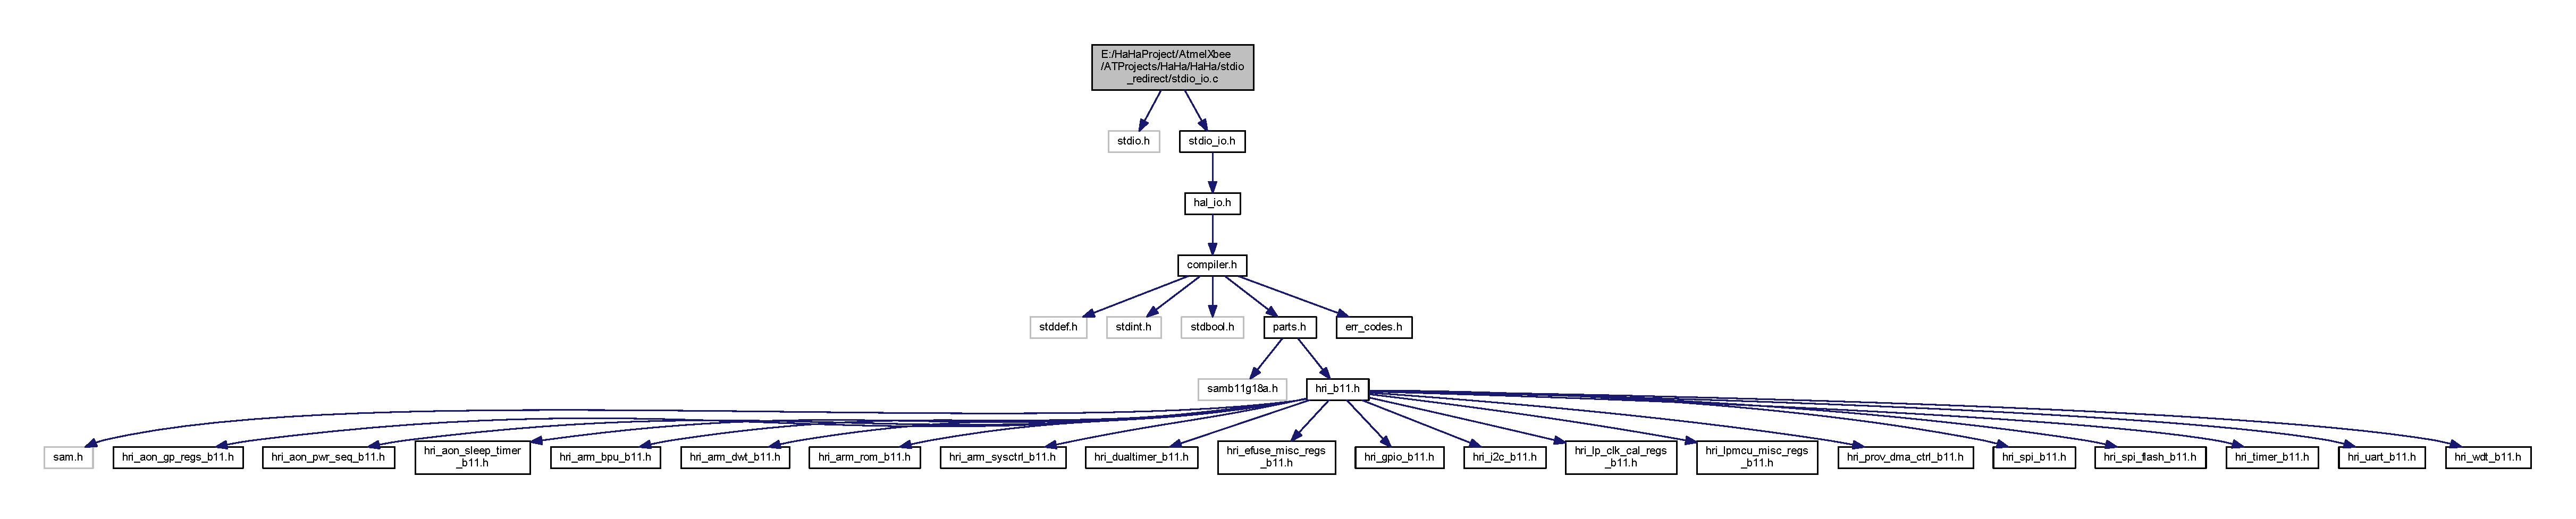
\includegraphics[width=350pt]{stdio__io_8c__incl}
\end{center}
\end{figure}
\subsection*{Functions}
\begin{DoxyCompactItemize}
\item 
void \hyperlink{stdio__io_8c_a832670dfdc8f3deb3b9b0a725c636409}{stdio\+\_\+io\+\_\+init} (struct \hyperlink{structio__descriptor}{io\+\_\+descriptor} $\ast$io)
\begin{DoxyCompactList}\small\item\em Initialize S\+T\+D\+IO access. \end{DoxyCompactList}\item 
void \hyperlink{stdio__io_8c_a31d48bd5f32a5ae99cc00a6ea7991a25}{stdio\+\_\+io\+\_\+set\+\_\+io} (struct \hyperlink{structio__descriptor}{io\+\_\+descriptor} $\ast$io)
\begin{DoxyCompactList}\small\item\em Change IO descriptor for terminal to R/W data. \end{DoxyCompactList}\item 
int32\+\_\+t \hyperlink{stdio__io_8c_ac791b192543d77c693e6ad6d63ce8a45}{stdio\+\_\+io\+\_\+read} (uint8\+\_\+t $\ast$buf, const int32\+\_\+t len)
\begin{DoxyCompactList}\small\item\em Read through specified terminal. \end{DoxyCompactList}\item 
int32\+\_\+t \hyperlink{stdio__io_8c_a01a0bad87561dd4fb0fef82f0419b1e1}{stdio\+\_\+io\+\_\+write} (const uint8\+\_\+t $\ast$buf, const int32\+\_\+t len)
\begin{DoxyCompactList}\small\item\em Write through specified terminal. \end{DoxyCompactList}\end{DoxyCompactItemize}


\subsection{Detailed Description}
S\+T\+D\+IO redirection terminal. 

Copyright (C) 2015 Atmel Corporation. All rights reserved.

\subsection{Function Documentation}
\mbox{\Hypertarget{stdio__io_8c_a832670dfdc8f3deb3b9b0a725c636409}\label{stdio__io_8c_a832670dfdc8f3deb3b9b0a725c636409}} 
\index{stdio\+\_\+io.\+c@{stdio\+\_\+io.\+c}!stdio\+\_\+io\+\_\+init@{stdio\+\_\+io\+\_\+init}}
\index{stdio\+\_\+io\+\_\+init@{stdio\+\_\+io\+\_\+init}!stdio\+\_\+io.\+c@{stdio\+\_\+io.\+c}}
\subsubsection{\texorpdfstring{stdio\+\_\+io\+\_\+init()}{stdio\_io\_init()}}
{\footnotesize\ttfamily void stdio\+\_\+io\+\_\+init (\begin{DoxyParamCaption}\item[{struct \hyperlink{structio__descriptor}{io\+\_\+descriptor} $\ast$}]{io }\end{DoxyParamCaption})}



Initialize S\+T\+D\+IO access. 


\begin{DoxyParams}[1]{Parameters}
\mbox{\tt in}  & {\em io} & Pointer to IO descriptor, N\+U\+LL to discard R/W without any error. \\
\hline
\end{DoxyParams}
\mbox{\Hypertarget{stdio__io_8c_ac791b192543d77c693e6ad6d63ce8a45}\label{stdio__io_8c_ac791b192543d77c693e6ad6d63ce8a45}} 
\index{stdio\+\_\+io.\+c@{stdio\+\_\+io.\+c}!stdio\+\_\+io\+\_\+read@{stdio\+\_\+io\+\_\+read}}
\index{stdio\+\_\+io\+\_\+read@{stdio\+\_\+io\+\_\+read}!stdio\+\_\+io.\+c@{stdio\+\_\+io.\+c}}
\subsubsection{\texorpdfstring{stdio\+\_\+io\+\_\+read()}{stdio\_io\_read()}}
{\footnotesize\ttfamily int32\+\_\+t stdio\+\_\+io\+\_\+read (\begin{DoxyParamCaption}\item[{uint8\+\_\+t $\ast$}]{buf,  }\item[{const int32\+\_\+t}]{len }\end{DoxyParamCaption})}



Read through specified terminal. 


\begin{DoxyParams}[1]{Parameters}
\mbox{\tt out}  & {\em buf} & Pointer to buffer to place read data \\
\hline
\mbox{\tt in}  & {\em len} & Data length in number of bytes \\
\hline
\end{DoxyParams}
\begin{DoxyReturn}{Returns}
status 
\end{DoxyReturn}

\begin{DoxyRetVals}{Return values}
{\em $>$=0} & number of bytes read \\
\hline
{\em $<$0} & error \\
\hline
\end{DoxyRetVals}
\mbox{\Hypertarget{stdio__io_8c_a31d48bd5f32a5ae99cc00a6ea7991a25}\label{stdio__io_8c_a31d48bd5f32a5ae99cc00a6ea7991a25}} 
\index{stdio\+\_\+io.\+c@{stdio\+\_\+io.\+c}!stdio\+\_\+io\+\_\+set\+\_\+io@{stdio\+\_\+io\+\_\+set\+\_\+io}}
\index{stdio\+\_\+io\+\_\+set\+\_\+io@{stdio\+\_\+io\+\_\+set\+\_\+io}!stdio\+\_\+io.\+c@{stdio\+\_\+io.\+c}}
\subsubsection{\texorpdfstring{stdio\+\_\+io\+\_\+set\+\_\+io()}{stdio\_io\_set\_io()}}
{\footnotesize\ttfamily void stdio\+\_\+io\+\_\+set\+\_\+io (\begin{DoxyParamCaption}\item[{struct \hyperlink{structio__descriptor}{io\+\_\+descriptor} $\ast$}]{io }\end{DoxyParamCaption})}



Change IO descriptor for terminal to R/W data. 


\begin{DoxyParams}[1]{Parameters}
\mbox{\tt in}  & {\em io} & Pointer to IO descriptor, N\+U\+LL to discard R/W without any error. \\
\hline
\end{DoxyParams}
\mbox{\Hypertarget{stdio__io_8c_a01a0bad87561dd4fb0fef82f0419b1e1}\label{stdio__io_8c_a01a0bad87561dd4fb0fef82f0419b1e1}} 
\index{stdio\+\_\+io.\+c@{stdio\+\_\+io.\+c}!stdio\+\_\+io\+\_\+write@{stdio\+\_\+io\+\_\+write}}
\index{stdio\+\_\+io\+\_\+write@{stdio\+\_\+io\+\_\+write}!stdio\+\_\+io.\+c@{stdio\+\_\+io.\+c}}
\subsubsection{\texorpdfstring{stdio\+\_\+io\+\_\+write()}{stdio\_io\_write()}}
{\footnotesize\ttfamily int32\+\_\+t stdio\+\_\+io\+\_\+write (\begin{DoxyParamCaption}\item[{const uint8\+\_\+t $\ast$}]{buf,  }\item[{const int32\+\_\+t}]{len }\end{DoxyParamCaption})}



Write through specified terminal. 


\begin{DoxyParams}[1]{Parameters}
\mbox{\tt in}  & {\em buf} & Pointer to buffer to place data to write \\
\hline
\mbox{\tt in}  & {\em len} & Data length in number of bytes \\
\hline
\end{DoxyParams}
\begin{DoxyReturn}{Returns}
status 
\end{DoxyReturn}

\begin{DoxyRetVals}{Return values}
{\em $>$=0} & number of bytes read \\
\hline
{\em $<$0} & error \\
\hline
\end{DoxyRetVals}

\hypertarget{stdio__io_8h}{}\section{E\+:/\+Ha\+Ha\+Project/\+Atmel-\/\+Xbee/\+A\+T\+Projects/\+Atmel\+\_\+\+Debug\+\_\+\+Xbee/\+Atmel\+\_\+\+Debug\+\_\+\+Xbee/stdio\+\_\+redirect/stdio\+\_\+io.h File Reference}
\label{stdio__io_8h}\index{E\+:/\+Ha\+Ha\+Project/\+Atmel-\/\+Xbee/\+A\+T\+Projects/\+Atmel\+\_\+\+Debug\+\_\+\+Xbee/\+Atmel\+\_\+\+Debug\+\_\+\+Xbee/stdio\+\_\+redirect/stdio\+\_\+io.\+h@{E\+:/\+Ha\+Ha\+Project/\+Atmel-\/\+Xbee/\+A\+T\+Projects/\+Atmel\+\_\+\+Debug\+\_\+\+Xbee/\+Atmel\+\_\+\+Debug\+\_\+\+Xbee/stdio\+\_\+redirect/stdio\+\_\+io.\+h}}


S\+T\+D\+IO redirection terminal.  


{\ttfamily \#include $<$hal\+\_\+io.\+h$>$}\newline
\subsection*{Functions}
\begin{DoxyCompactItemize}
\item 
void \hyperlink{stdio__io_8h_a832670dfdc8f3deb3b9b0a725c636409}{stdio\+\_\+io\+\_\+init} (struct io\+\_\+descriptor $\ast$io)
\begin{DoxyCompactList}\small\item\em Initialize S\+T\+D\+IO access. \end{DoxyCompactList}\item 
void \hyperlink{stdio__io_8h_a31d48bd5f32a5ae99cc00a6ea7991a25}{stdio\+\_\+io\+\_\+set\+\_\+io} (struct io\+\_\+descriptor $\ast$io)
\begin{DoxyCompactList}\small\item\em Change IO descriptor for terminal to R/W data. \end{DoxyCompactList}\item 
int32\+\_\+t \hyperlink{stdio__io_8h_ac791b192543d77c693e6ad6d63ce8a45}{stdio\+\_\+io\+\_\+read} (uint8\+\_\+t $\ast$buf, const int32\+\_\+t len)
\begin{DoxyCompactList}\small\item\em Read through specified terminal. \end{DoxyCompactList}\item 
int32\+\_\+t \hyperlink{stdio__io_8h_a01a0bad87561dd4fb0fef82f0419b1e1}{stdio\+\_\+io\+\_\+write} (const uint8\+\_\+t $\ast$buf, const int32\+\_\+t len)
\begin{DoxyCompactList}\small\item\em Write through specified terminal. \end{DoxyCompactList}\end{DoxyCompactItemize}


\subsection{Detailed Description}
S\+T\+D\+IO redirection terminal. 

Copyright (C) 2015 Atmel Corporation. All rights reserved.

\subsection{Function Documentation}
\mbox{\Hypertarget{stdio__io_8h_a832670dfdc8f3deb3b9b0a725c636409}\label{stdio__io_8h_a832670dfdc8f3deb3b9b0a725c636409}} 
\index{stdio\+\_\+io.\+h@{stdio\+\_\+io.\+h}!stdio\+\_\+io\+\_\+init@{stdio\+\_\+io\+\_\+init}}
\index{stdio\+\_\+io\+\_\+init@{stdio\+\_\+io\+\_\+init}!stdio\+\_\+io.\+h@{stdio\+\_\+io.\+h}}
\subsubsection{\texorpdfstring{stdio\+\_\+io\+\_\+init()}{stdio\_io\_init()}}
{\footnotesize\ttfamily void stdio\+\_\+io\+\_\+init (\begin{DoxyParamCaption}\item[{struct io\+\_\+descriptor $\ast$}]{io }\end{DoxyParamCaption})}



Initialize S\+T\+D\+IO access. 


\begin{DoxyParams}[1]{Parameters}
\mbox{\tt in}  & {\em io} & Pointer to IO descriptor, N\+U\+LL to discard R/W without any error. \\
\hline
\end{DoxyParams}
\mbox{\Hypertarget{stdio__io_8h_ac791b192543d77c693e6ad6d63ce8a45}\label{stdio__io_8h_ac791b192543d77c693e6ad6d63ce8a45}} 
\index{stdio\+\_\+io.\+h@{stdio\+\_\+io.\+h}!stdio\+\_\+io\+\_\+read@{stdio\+\_\+io\+\_\+read}}
\index{stdio\+\_\+io\+\_\+read@{stdio\+\_\+io\+\_\+read}!stdio\+\_\+io.\+h@{stdio\+\_\+io.\+h}}
\subsubsection{\texorpdfstring{stdio\+\_\+io\+\_\+read()}{stdio\_io\_read()}}
{\footnotesize\ttfamily int32\+\_\+t stdio\+\_\+io\+\_\+read (\begin{DoxyParamCaption}\item[{uint8\+\_\+t $\ast$}]{buf,  }\item[{const int32\+\_\+t}]{len }\end{DoxyParamCaption})}



Read through specified terminal. 


\begin{DoxyParams}[1]{Parameters}
\mbox{\tt out}  & {\em buf} & Pointer to buffer to place read data \\
\hline
\mbox{\tt in}  & {\em len} & Data length in number of bytes \\
\hline
\end{DoxyParams}
\begin{DoxyReturn}{Returns}
status 
\end{DoxyReturn}

\begin{DoxyRetVals}{Return values}
{\em $>$=0} & number of bytes read \\
\hline
{\em $<$0} & error \\
\hline
\end{DoxyRetVals}
\mbox{\Hypertarget{stdio__io_8h_a31d48bd5f32a5ae99cc00a6ea7991a25}\label{stdio__io_8h_a31d48bd5f32a5ae99cc00a6ea7991a25}} 
\index{stdio\+\_\+io.\+h@{stdio\+\_\+io.\+h}!stdio\+\_\+io\+\_\+set\+\_\+io@{stdio\+\_\+io\+\_\+set\+\_\+io}}
\index{stdio\+\_\+io\+\_\+set\+\_\+io@{stdio\+\_\+io\+\_\+set\+\_\+io}!stdio\+\_\+io.\+h@{stdio\+\_\+io.\+h}}
\subsubsection{\texorpdfstring{stdio\+\_\+io\+\_\+set\+\_\+io()}{stdio\_io\_set\_io()}}
{\footnotesize\ttfamily void stdio\+\_\+io\+\_\+set\+\_\+io (\begin{DoxyParamCaption}\item[{struct io\+\_\+descriptor $\ast$}]{io }\end{DoxyParamCaption})}



Change IO descriptor for terminal to R/W data. 


\begin{DoxyParams}[1]{Parameters}
\mbox{\tt in}  & {\em io} & Pointer to IO descriptor, N\+U\+LL to discard R/W without any error. \\
\hline
\end{DoxyParams}
\mbox{\Hypertarget{stdio__io_8h_a01a0bad87561dd4fb0fef82f0419b1e1}\label{stdio__io_8h_a01a0bad87561dd4fb0fef82f0419b1e1}} 
\index{stdio\+\_\+io.\+h@{stdio\+\_\+io.\+h}!stdio\+\_\+io\+\_\+write@{stdio\+\_\+io\+\_\+write}}
\index{stdio\+\_\+io\+\_\+write@{stdio\+\_\+io\+\_\+write}!stdio\+\_\+io.\+h@{stdio\+\_\+io.\+h}}
\subsubsection{\texorpdfstring{stdio\+\_\+io\+\_\+write()}{stdio\_io\_write()}}
{\footnotesize\ttfamily int32\+\_\+t stdio\+\_\+io\+\_\+write (\begin{DoxyParamCaption}\item[{const uint8\+\_\+t $\ast$}]{buf,  }\item[{const int32\+\_\+t}]{len }\end{DoxyParamCaption})}



Write through specified terminal. 


\begin{DoxyParams}[1]{Parameters}
\mbox{\tt in}  & {\em buf} & Pointer to buffer to place data to write \\
\hline
\mbox{\tt in}  & {\em len} & Data length in number of bytes \\
\hline
\end{DoxyParams}
\begin{DoxyReturn}{Returns}
status 
\end{DoxyReturn}

\begin{DoxyRetVals}{Return values}
{\em $>$=0} & number of bytes read \\
\hline
{\em $<$0} & error \\
\hline
\end{DoxyRetVals}

%--- End generated contents ---

% Index
\backmatter
\newpage
\phantomsection
\clearemptydoublepage
\addcontentsline{toc}{chapter}{Index}
\printindex

\end{document}
